\section{Artificial Intelligence}
Challenging gameplay is an requirement of the game since it keeps the user in the flow zone. %ref to flowzone shizzle
The AI in \#GAME is what makes the game challenging so therefore we have to develop some kind of AI which can be a threat to the player. 

To make the enemies more challenging they would have to go towards the player without getting stuck on a static obstacle.
This could be achieved by applying a pathfinding algorithm to the AI's behaviour.

The pathfinding algorithm that we will be using is A* search pathfinding which has a runtime of [].
%Other pathfinding possibilities would be BFS or floyd-warshall algorithm, but as BFS has a runtime of [] and floyd-warshall has a runtime of [] with a high memory usage, we will not be using them.

The first step in using an A* search algorithm, is to have a proper graph which represents the level in the game.
Our initial idea was to simply have each walkable square in the grid to be a node.
A node would then have up to eight connections which would point to a neighbour of that certain node with a cost of traversing to this node.
Possible neighbours would be four to each side of the node with a cost of 10 and four diagonal neighbours with a cost of 14.
This approach resulted in a very large graph which took a lot of time to create and traverse through, when running the algorithm on it.
An example of this can be seen in figure \ref{gridGraph} where you can see a level of size 64x64, the graph created for that level has 3984 nodes and 30450 edges.

An optimisation for to this was to change the graph from being grid based to a waypoint graph.
We would create the graph based on the outer corners of the obstacles on the map, where the AI had to make a turn, as seen in figure \ref{waypointsNode}.
Each point would then do a check on every other point to see if it was in direct sight, if that was the case it was added as a neighbour and the cost for that edge would be the euclidean distance to that point.
A resulting graph can be seen in figure \ref{waypointgraph}.
This approach resulted in a much smaller graph with 47 nodes and 624 edges, thus improving both the creation of the graph and the traversal of it.

Running the A* search pathfinding from every enemy is very costly, and as of such we will have to make some cheap optimisations to avoid that.
First optimisation is to check whether the player is in direct sight which means we can go straight towards the player and not run any pathfinding algorithm.
If the player then runs out of sight, we can still continue to walk towards the position where the player was last seen and once we have reached that position we look for the player again.
When the player is not in sight, we check for surrounding enemies who perhaps have run the pathfinding algorithm and are on their way towards the player, then we simply follow this entity.
When neither of the above options are available, we run the pathfinding algorithm and follow the path until we have the player in sight again or reached the end of the path where we then have to run the algorithm again.



%Gridbased graph: 3984 nodes, 30450 edges
%Waypoint graph: 47 nodes, 624 edges

\begin{figure}
	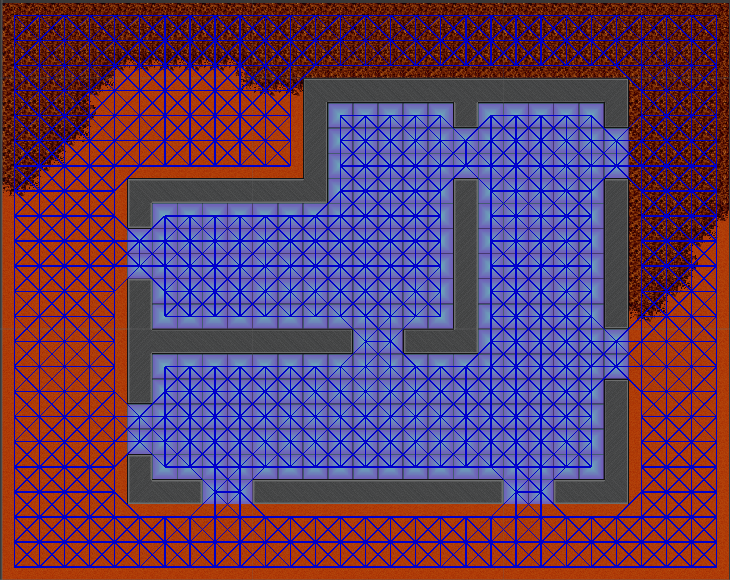
\includegraphics[width=\textwidth]{figures/astar/gridGraph}
	\caption{Somegraph....}
	\label{gridGraph}
\end{figure}

\begin{figure}
	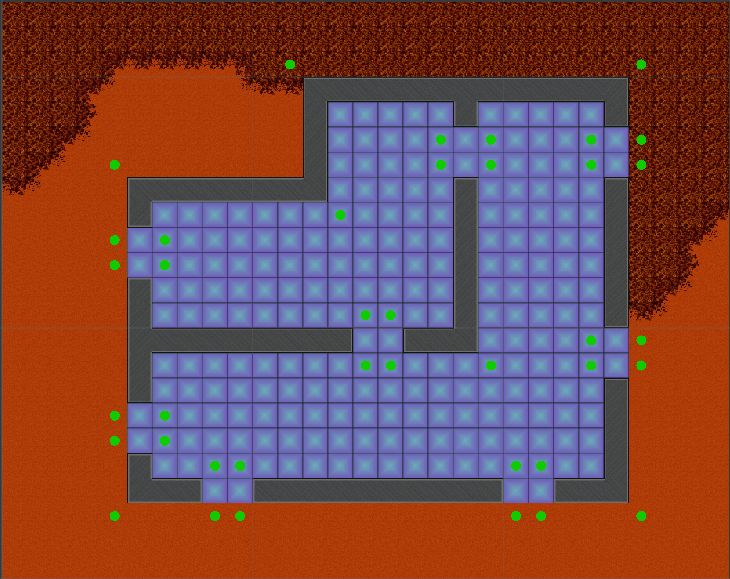
\includegraphics[width=\textwidth]{figures/astar/waypoints}
	\caption{Somegraph....}
	\label{waypointsNode}
\end{figure}

\begin{figure}
	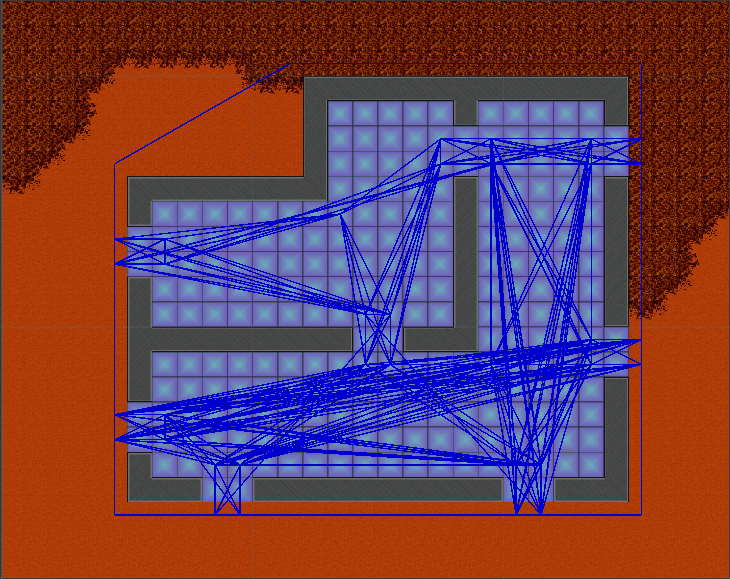
\includegraphics[width=\textwidth]{figures/astar/waypointsGraph}
	\caption{Somegraph....}
	\label{waypointgraph}
\end{figure}
